\documentclass[12ptj,a4j,dvipdfmx,uplatex, titlepage]{jsarticle}

% \enhanceでボールドゴシック
\newcommand{\enhance}[1]{{\textbf{\gtfamily\sffamily#1}}}

% レイアウト
\usepackage[driver=dvipdfm,hmargin=19.05truemm,vmargin=25.40truemm]{geometry}

% エンコーディング
\usepackage[T1]{fontenc}

% 日本語フォント
\usepackage[expert,deluxe,uplatex]{otf}

% 数式・科学表記
\usepackage{amsmath,amssymb,bm,mleftright,diffcoeff}
\usepackage{siunitx}

% 画像処理
\usepackage[dvipdfmx]{graphicx}

% 参考文献スタイル指定
\usepackage[nobreak]{cite}
\usepackage[resetlabels]{multibib}
\newcites{pubs}{発表文献}
\bibliographystyle{junsrt} %jplain
\bibliographystylepubs{junsrt}
\nocitepubs{*}

% 相互参照
\usepackage[hidelinks]{hyperref}

% URL
\usepackage{url}


% 画像用ディレクトリ
\graphicspath{{images/}}

\title{卒業論文中間報告書\vspace{1em}\\歌声の音高と音素の発声しやすさとの\\関係について}

\author{03-180480 小林海斗\vspace{1em}\\峯松・齋藤研究室}

\date{2019年9月30日}
%%
%% main
%%
\begin{document}

\maketitle

\tableofcontents
\clearpage

\section{はじめに}
近年、カラオケが一般的な娯楽となっており、歌を歌うことも身近なものとなっている。
人間は歌う際に、声の高さを適切に制御することで特定の旋律を表現する。しかし、
出せる声の高さには限界がある。また、
高音域を歌う際に母音が「i」だと途端に歌いにくくなるという経験は想像に難くない。
歌詞の点からみてもサビにおける高音の「i」の頻度は「a」に比べて低く\cite{popular_highest}、作詞段階で意図的に
避けられていると考えられる。
この発声難度の違いの定量的な知見が得られれば、歌詞作成など様々な応用が考えられる。
しかし、この違いはこれまで定量的に分析されていなかった。そこで、ここでは
この違いを定量的に分析する様々な手法について検討する。
分析にはいくつかの手法があるが、ここでは母音と関連の深いフォルマント周波数や、音色を
表す声道特徴量に着目する。
また、人間の声の高さの物理的制約にも分析するため、声帯の機構についても検討する。

第2章では母音とフォルマント周波数がどのように関連しているか説明し、
第3章では音高と声帯周辺の筋肉の関係を説明する。
そして第4章でいくつかの分析方法を示し、第5章で研究の方針を示す。

\section{母音とフォルマント周波数}
母音の音声は、肺からの空気が声帯を振動させ、声道を通過して音響的に整形されることで生じる。
ここで声帯振動による音を喉頭音源とよぶ。
声道は共鳴器であり、フォルマント周波数周辺の音は他よりも強い音となって口唇から伝播する。

声道の形状を、声門への距離に応じて変化する断面積の関数として考えると、声道の形状は曲線として記述できる。
これを声道断面積関数とよぶ\cite{science}。
\begin{figure}[htbp]
    \begin{center}
      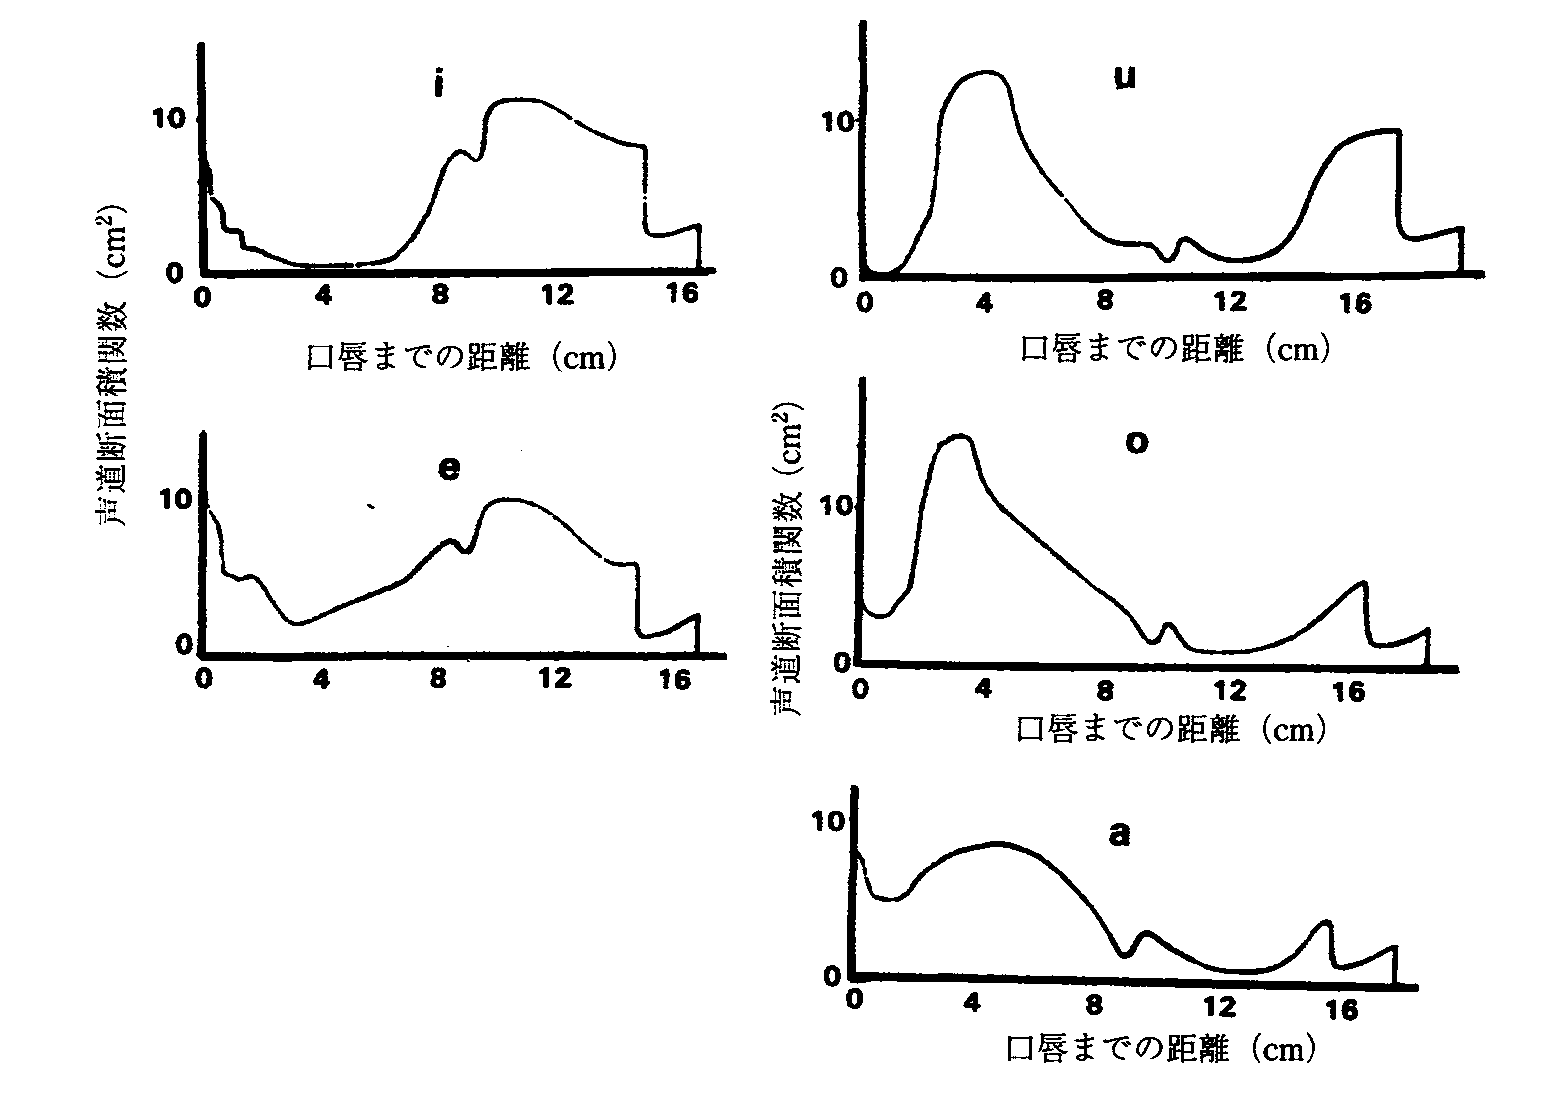
\includegraphics[clip,width=12.0cm]{声道断面積関数.png}
      \caption{断面積関数\cite{science}}
      \label{fig:danmen}
    \end{center}
  \end{figure}

フォルマント周波数は母音や声質の決定において非常に重要である。
フォルマント周波数は声道スペクトルのピークとなる共鳴周波数のことであり、
低い方から順に第1フォルマント(F1)、第2フォルマント(F2)、と名付けられる。

調音器官の運動は、フォルマント周波数全てに影響を与える。
第1フォルマントは顎の開きに敏感で、開き具合が大きくなるほど第1フォルマント周波数は上昇する。
第2フォルマントは特に舌の形状に大きく影響を受ける。
声道前方を狭めるときに第2フォルマント周波数はもっとも高くなる。
逆に、軟口蓋や咽頭部を狭める時には低くなる。
第3フォルマントは舌尖の位置、正確には前歯のすぐ後ろの空間に影響を受ける。
空間が大きいほど第3フォルマント周波数は低くなる。

フォルマント周波数のうち特にF1、F2は母音を特徴付ける重要なパラメータであり、これらの分布によって母音を分類することができる\cite{japanese_vowels}。
図\ref{fig:jp_formant}は日本語5母音の第1、第2フォルマント周波数を示したものである。

\begin{figure}[htbp]
    \begin{center}
      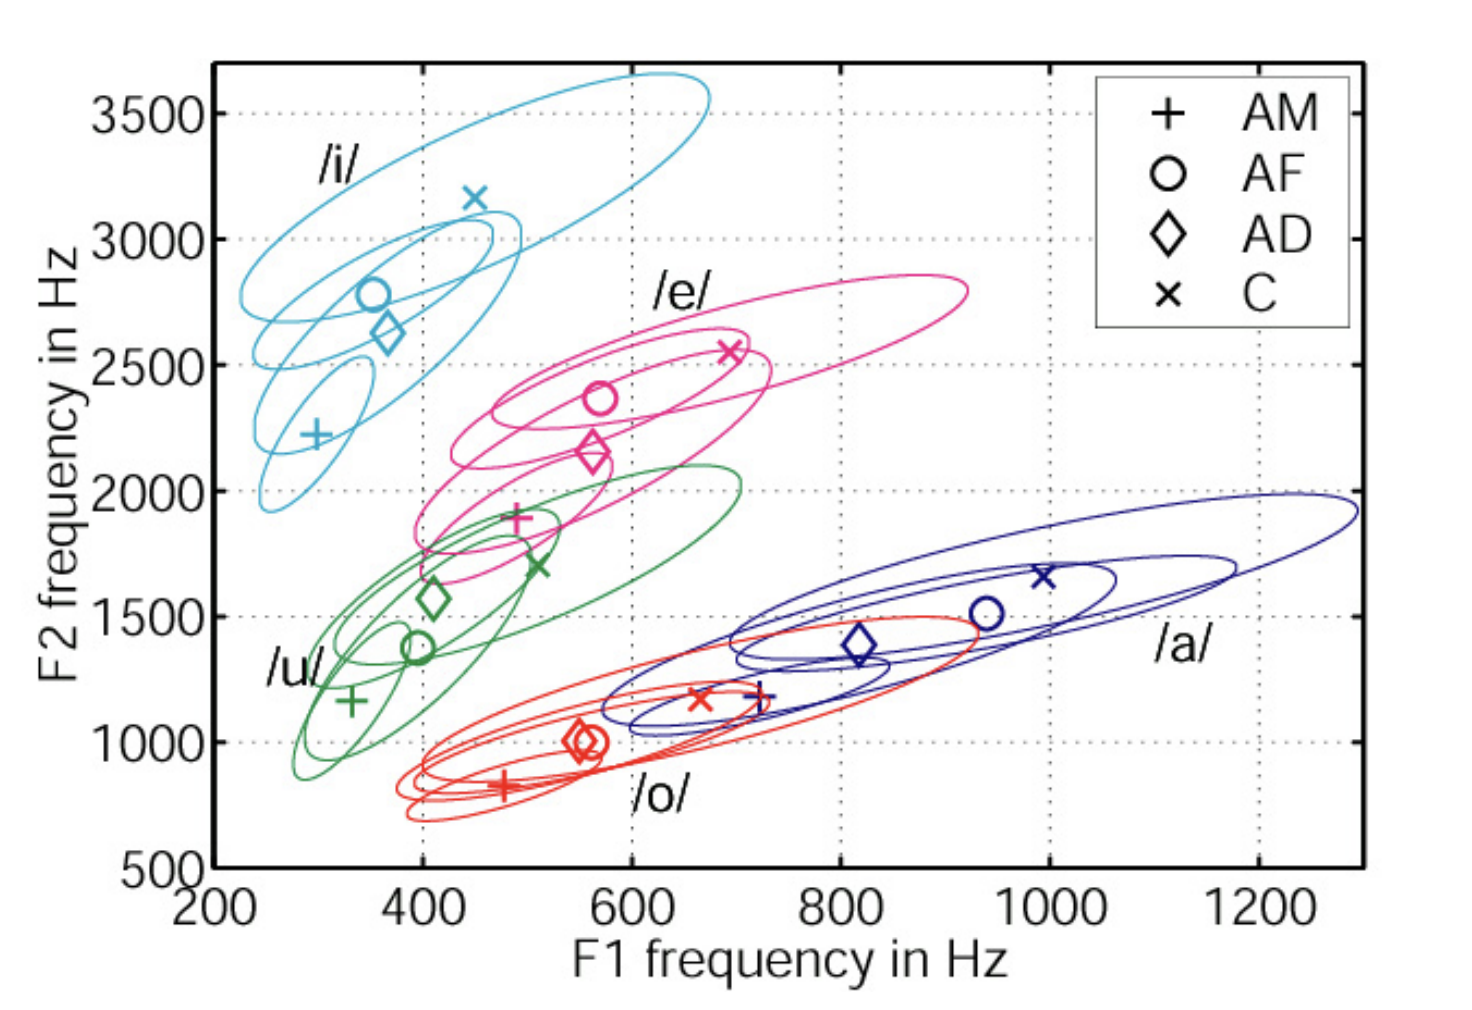
\includegraphics[clip,width=7.0cm]{5母音.png}
      \caption{日本語5母音の第1、第2フォルマント周波数\cite{japanese_vowels}}
      \label{fig:jp_formant}
    \end{center}
  \end{figure}
  ここでAMは成人男性、AFは成人女性、ADは青年、Cは子供である。一般に、平均的な声が高いほど
  フォルマント周波数も高い傾向にある。
  成人男性を例に挙げると、第1フォルマントは250〜1000 \si{Hz}、第2フォルマントは600〜2500 \si{Hz}、
  第3フォルマントは1700〜3500 \si{Hz}である\cite{science}。





母音「a」では口唇側が大きく、声門側が小さい一方、母音「i」では口唇側が小さく、声門側が大きい。
また、母音「a」のF1は高く、F2は低い一方、母音「i」のF1は低く、F2は高い。
このように、声道形状とF1、F2の関係はよく知られており、舌の高さとF1、舌の前後方向の位置とF2にはそれぞれ相関がある\cite{katei}。

調音器官には口唇、舌の他に顎、喉頭なども含まれる。これらは連動して動くため、1つの調音器官のみを変化させて考えるのは適切でない。
\begin{figure}[htbp]
    \begin{center}
      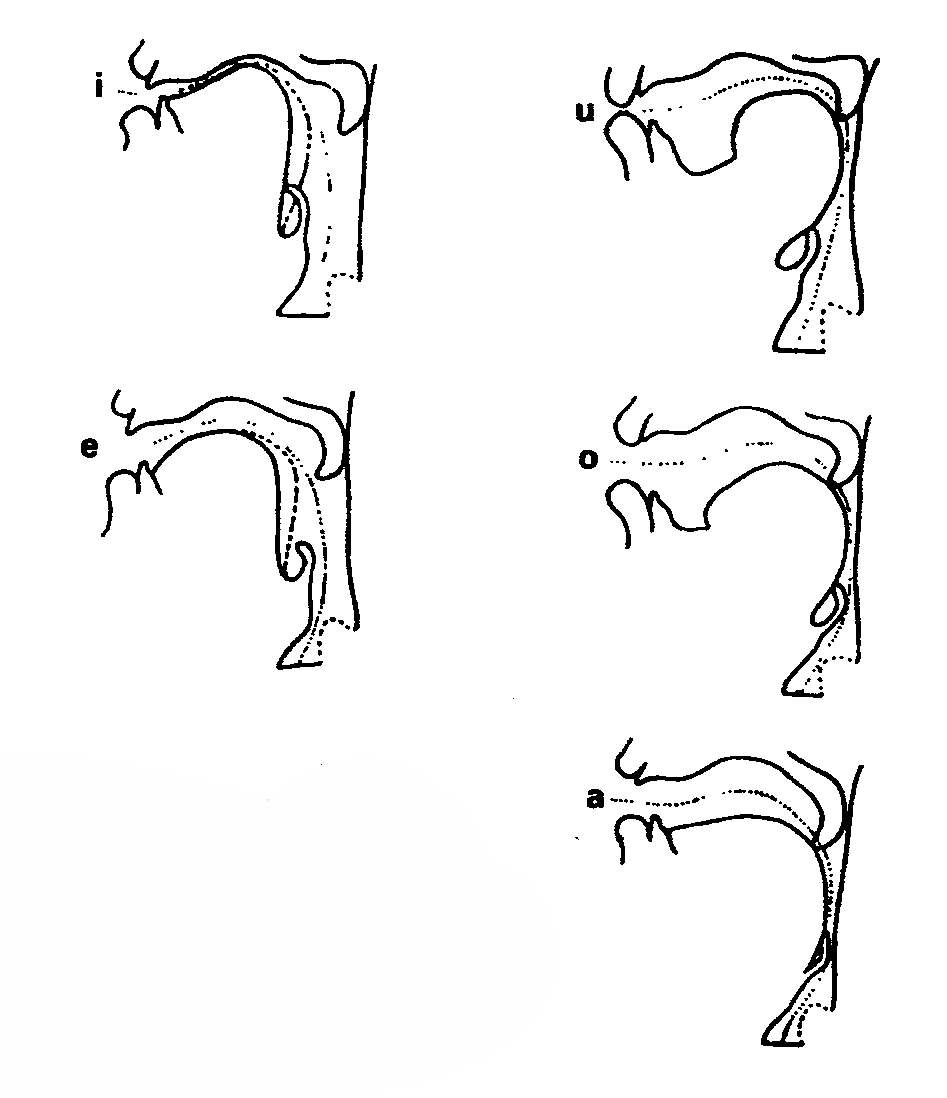
\includegraphics[clip,width=7.0cm]{声道形状.png}
      \caption{声道の輪郭\cite{science}}
      \label{fig:seido}
    \end{center}
\end{figure}

\section{喉頭音源の制御と音高}
発声周波数は、声帯の張力と厚みによって決まる。ここで張力は声帯長を操作して変化する。そのため、
ピッチが低い時声帯は厚く短くなっており、逆にピッチが高い時声帯は薄く長くなっている。
この声帯長の変化は、主に輪状甲状筋の収縮によって引き起こされる(図\ref{fig:rinjo})。

\begin{figure}[htbp]
    \begin{center}
      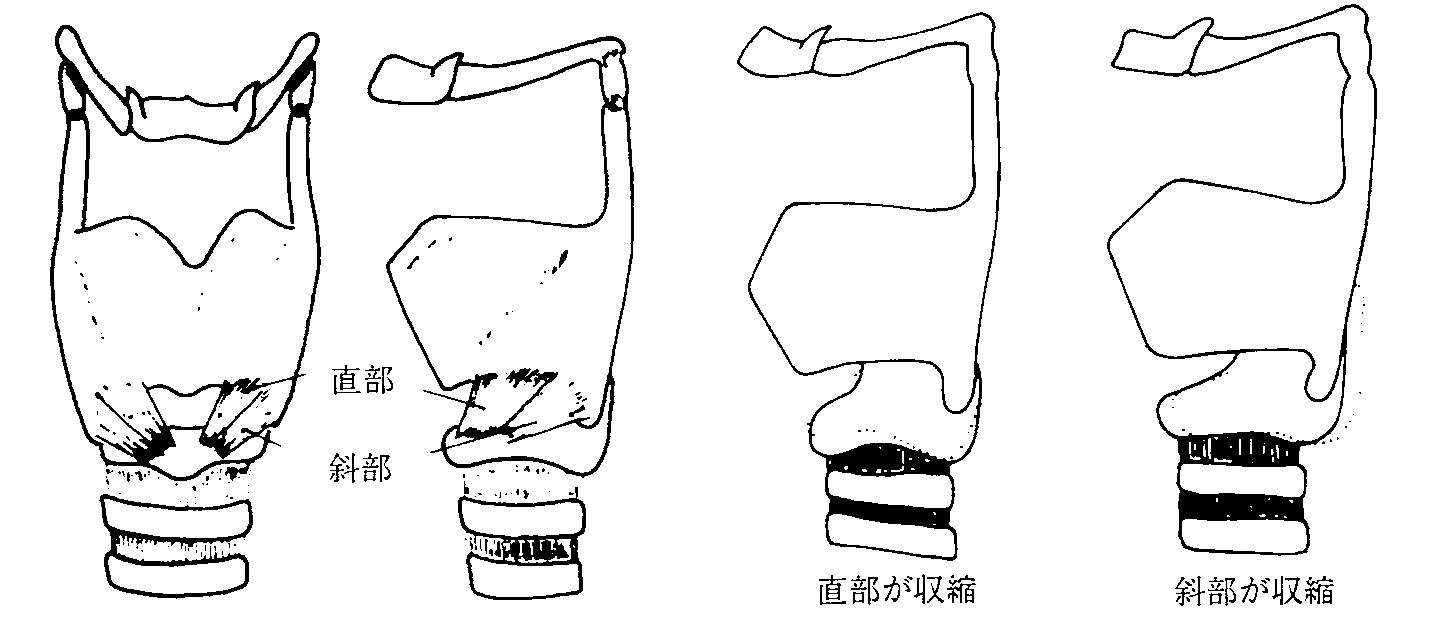
\includegraphics[clip,width=10.0cm]{輪状甲状筋.png}
      \caption{輪状甲状筋の機能\cite{science}}
      \label{fig:rinjo}
    \end{center}
\end{figure}

輪状甲状筋は直部と斜部に分かれている。
直部の収縮は輪状軟骨を傾け、それにより輪状軟骨と甲状軟骨の距離を短くする。
その結果甲状軟骨と披裂軟骨との距離が長くなり、声帯を伸展させる。
斜部の収縮は、輪状軟骨を前方に動かし、甲状軟骨と輪状軟骨の距離を大きくすることで声帯を伸展させる。

また、喉頭は「i」のように口唇を横に引っ張って発声する時に上昇し、
「u」のように円唇母音の時に下降する。
喉頭の位置は発声周波数によっても変化し、一般に周波数が高いほど喉頭の位置も高くなる(図\ref{fig:koto})。

\begin{figure}[htbp]
    \begin{center}
      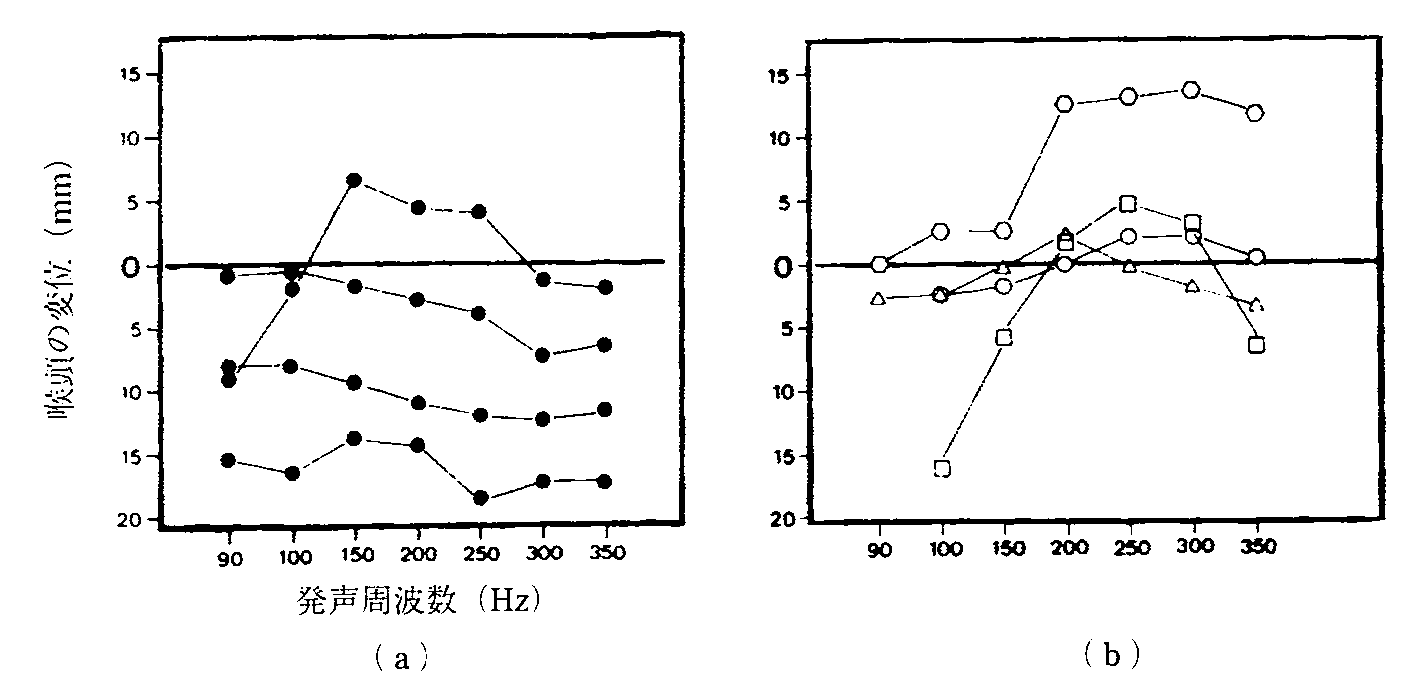
\includegraphics[clip,width=12.0cm]{喉頭位置.png}
      \caption{男性歌手(a)と歌手でない男性(b)における、発声周波数ごとの垂直方向の喉頭の位置\cite{science}}
      \label{fig:koto}
    \end{center}
\end{figure}

歌手でない男性の喉頭位置の変化(b)を見ると、位置は人により様々であるが、200 \si{Hz}までは喉頭位置が発声周波数の上昇に
したがって上昇している。
(a)はプロの歌手の結果であり、(b)と比べると大きく異なっている。一般に喉頭位置が発声周波数の上昇に伴って
下降しているといえる。
このように喉頭の位置は発声周波数にある程度関係しているが、意図的にコントロールすることも可能である。



\section{声道特徴量の分析手法}

音声は、喉頭音源と声道によって生成される。音色の特性に着目するには声道特徴量も重要である。
母音ごとの特徴を見るのであればこれらの特性を分離すると都合が良い。
声道特徴量の分析にはケプストラム分析やLPC分析がある。これらについて説明していく。

\subsection{ケプストラム分析}
ケプストラム分析とは、喉頭音源特性と声道特性を分離して、スペクトル包絡を求める手法である。
まず音声波形データに下処理(後述)を施したのちフーリエ変換する。
次に、各周波数量の対数をとってデシベル表記に変換する。
これを逆フーリエ変換しケプストラム領域に移すことで、喉頭音源特性と声道特性を分離できる。
ここで低次のケプストラムは声道特性(スペクトル包絡)に、
高次のケプストラムは喉頭音源特性(スペクトル微細構造)に対応しているため、
低次のみを取り出すことで包絡を抽出することができる。

これは以下のように説明できる。
喉頭音源を$g(t)$、声道断面積関数を$h(t)$とすると、出力信号は$g(t)$、$h(t)$の畳み込み積分
\begin{equation}
    x(t) = g(t) * h(t)
\end{equation}
とかける。
これは周波数領域では$G(\Omega)$、$H(\Omega)$を用いて、
\begin{equation}
    X(\Omega) = G(\Omega) \times H(\Omega)
\end{equation}
とかける。対数をとることで
\begin{equation}
    \log |X(\Omega)| = \log |G(\Omega)| + \log |H(\Omega)|
\end{equation}
となり、確かに分離できることがわかる。


なお、FFTを行う前に下処理として高域強調処理、窓関数適用を行う。

\subsubsection{高域強調処理}
音声パワーは広域になるほど減衰するため、高域強調処理を行う。一般には6 \si{dB/oct}の強調となるように行う。
高域通過フィルタとしては以下のような1次有限インパルス応答フィルタ$H(z)$が用いられる。
\begin{equation}
    H(z) = 1 - \alpha z^{-1}
\end{equation}

ここで$z= \exp(j\omega)$、$\omega = 2\pi f/f_s$で、$f$は周波数、$f_s$はサンプリング周波数である。

量子化された離散信号においては
\begin{equation}
    y(n) = x(n) - \alpha x(n-1)
\end{equation}
と表す。$\alpha$ の値としては0.97がよく用いられる。

\subsubsection{窓関数}
FFTは周期関数に対して適用するが、一般の音声データは周期的になっておらず両端が不連続であり、
このまま分析を行うと高周波に雑音が乗ってしまう。
そこで、波形に対して両端が減衰するように分析窓をかける。
分析窓としてはハミング窓とハニング窓が知られており、それぞれ以下の式で表せる。
\begin{eqnarray}
    W_H (n) &=& 0.54 - 0.46 \cos \frac{2n\pi}{N-1} \\
    W_N (n) &=& 0.5 - 0.5 \cos \frac{2n\pi}{N-1}
\end{eqnarray}

ただし$n$が0未満あるいは$N$以上の時はゼロの値をとる。
多くの場合は前者のハミング窓が用いられる。

\subsubsection{MFCC}
MFCC(メル周波数ケプストラム係数)は人間の聴覚の特性に基づく分析手法であり、主に音声認識分野で使われる\cite{onsei}。

人間は音が高くなるにつれて音高の変化を小さく感じてしまう。そこで用いられる尺度がメル尺度であり、
1000 \si{Hz}を基準としてその$n$倍に知覚する周波数を$n\times 1000$ \si{mel}と表す。
いくつかの種類のうち、よく使われるのが以下のファントの式である。
\begin{equation}
    m = \frac{1000}{\log_{10} 2} \log_{10} \left( \frac{f}{1000}+1 \right)
\end{equation}

これを適用するために、メルフィルタバンクをかける。
これはファントの式に合わせた尺度で周波数軸をとり、その上で幅が均等になるようにフィルタを割り振っている(図\ref{fig:mfcc})。
\begin{figure}[htbp]
    \begin{center}
      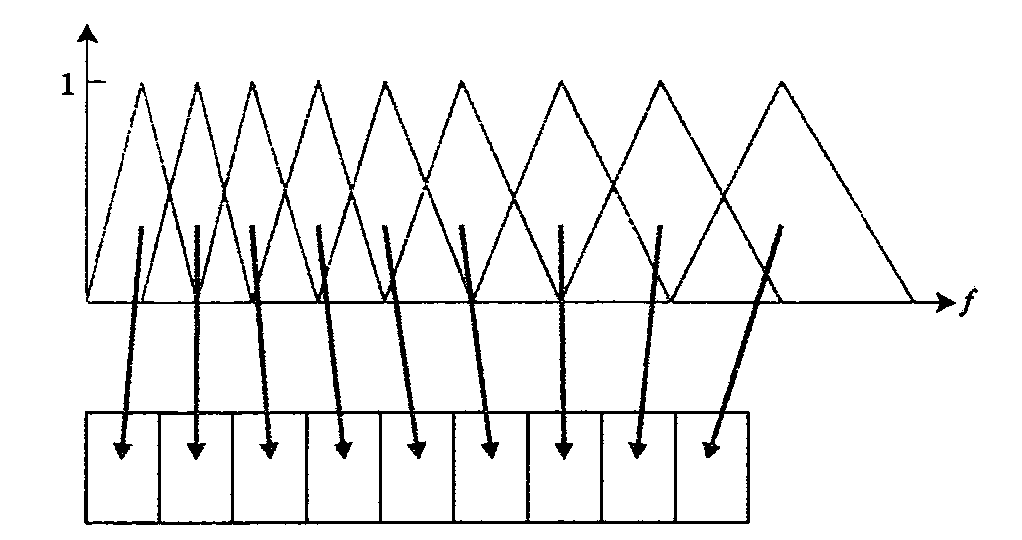
\includegraphics[clip,width=7.0cm]{MFCC.png}
      \caption{メルフィルタバンク\cite{onsei}}
      \label{fig:mfcc}
    \end{center}
\end{figure}

これ以降の手順は上記のケプストラム分析と同様である。

\subsection{LPC分析}
ケプストラム分析とは別の手法として、線形予測分析(LPC)がある\cite{lpc}。
まず声道フィルタを、極のみをもち零をもたないフィルタで近似する。
\begin{equation}
    H(z) = \frac{1}{\prod^p _{i=1} \left( 1-\frac{z}{z_i} \right)} 
    = \frac{1}{\sum_{k=0}^p \alpha_k z^{-k}}
\end{equation}

ただし、$\alpha_0 = 1$である。伝達関数の式$H(z) = G(z)H(z)$に代入すると、
\begin{equation}
    X(z) \left( \sum_{k=0}^p \alpha_k z^{-k} \right) = G(z)
\end{equation}
となり、両辺を逆Z変換すると、
\begin{equation}
    x[n] + \alpha_1 x[n-1] + \cdots + \alpha_p x[n-p] = g[n]
\end{equation}
となる。したがって、音声信号は
\begin{equation}
    x[n] = -\sum_{k=1}^p \alpha_k x[n-k] + g[n]
\end{equation}
と表せる。

右辺第1項を$\hat{x}_p[n]$と置き、第2項を$\epsilon[n]$と置き換えると、
\begin{equation}
    x[n] = \hat{x}_p[n] + \epsilon[n]
\end{equation}
となる。これは、現在の出力が過去の出力の線型結合$\hat{x}_p[n]$と残差$\epsilon[n]$の和で書けることを意味する。
線形予測分析はこの誤差のパワーが小さくなるように$\alpha_k$の値を調整し、スペクトルを近似することだといえる。

\subsection{分析手法の比較}

ケプストラム分析とLPC分析を比較したものが図\ref{fig:hikaku}である。

\begin{figure}[htbp]
    \begin{center}
      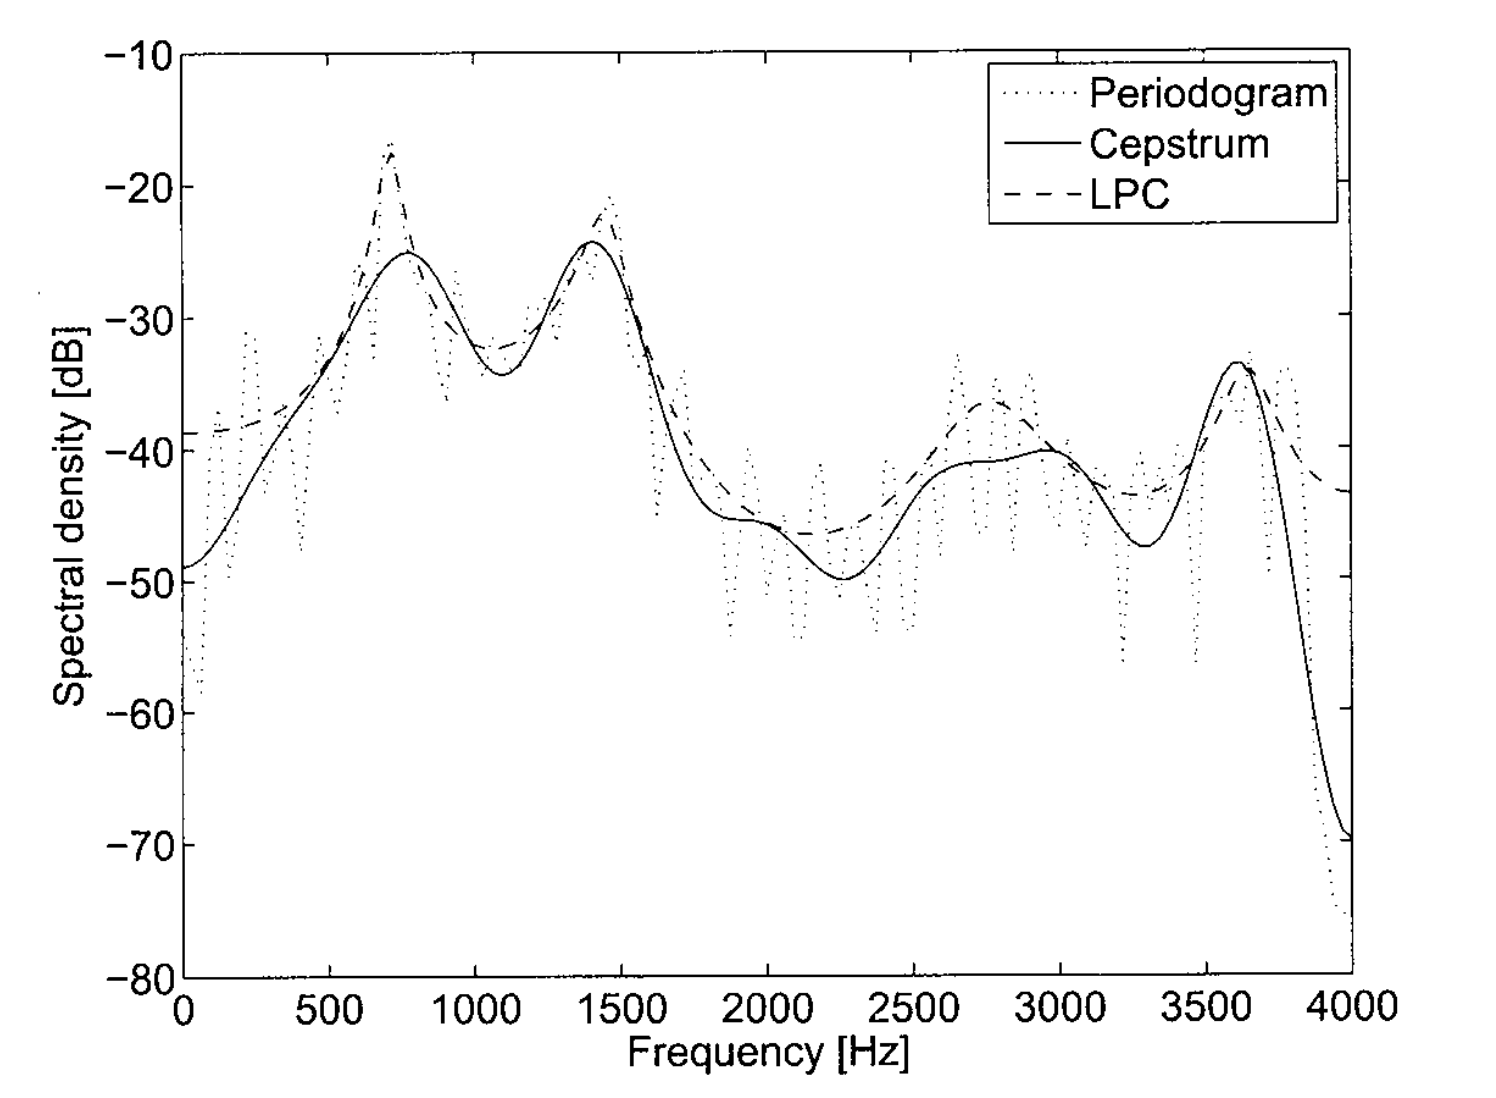
\includegraphics[clip,width=7.0cm]{比較.png}
      \caption{分析結果の比較\cite{lpc}}
      \label{fig:hikaku}
    \end{center}
\end{figure}

ケプストラム分析では音声の山も谷も同様に平滑化しているが、LPCでは山をより重視したものとなっていることがわかる。
この違いを把握した上で、適切な分析方法を選択する必要がある。



\section{今後の展望}
本研究では、歌声の基本周波数の変化が声道特性と喉頭音源特性の片方あるいは両方に影響を及ぼすと仮定して
実験しようと考えている。

その上で、「発声しやすさ」という主観的な特徴を、声道特性や喉頭音源特性に見出すことが第1の目標である。

具体的にはケプストラム分析、LPC分析を用いて声道特性を求め、母音ごとに音高を変えた時のスペクトルを比較し、
スペクトルやフォルマント周波数への影響を見ていく。

また、歌に熟達した者とそうでない者それぞれのデータを収集し比較することで、どのパラメータが「発声しやすさ」に影響しているかを
考察する。

フォルマント周波数を測定するために、まずはフリーソフトウェアのPraatを用いて研究を行う\cite{praat}。
Praatは、アムステルダム大学のPaul Boersma、David Weeninkによって開発されたオープンソースのソフトウェアである。

喉頭音源特性や声道特性は男性と女性、また子供と大人で大きく変わるため、まずは成人男性に限定して研究を行う。
歌唱経験の有無も結果に関わってくると考えられるため、歌唱経験の長い者、短い者それぞれに対して調査する。
測定音域はF3からA4までの範囲を想定している。一般男性における地声、地声と裏声の喚声点付近、ミックスボイスが
全て含まれるように設定している。
これらを母音「a」「i」「u」「e」「o」それぞれにおいて測定し、音高の変化にしたがってフォルマント周波数がどのように変化するかを
みる。
単音では歌唱時の発声かどうか曖昧なため、旋律に母音を乗せて歌唱させる。
歌唱後、発声のしやすさを主観的に「出しやすい」「やや出しやすい」「やや出しにくい」「出しにくい」の4段階で評価させる。
評価の基準として、最も出しやすい音高での「a」の母音を「出しやすい」とする。

得られた音声からF0やフォルマント周波数、MFCCなどの特徴量を抽出し、
さらに主観評価の結果を用いて分析を行う。
フォルマント周波数は母音を決定づけるF1、F2以外に、声質を決定づけるF3以上の値にも着目する。

\bibliography{references}
\end{document}